\documentclass[a4paper,UTF8]{article}
\usepackage{ctex}
\usepackage[margin=1.25in]{geometry}
\usepackage{color}
\usepackage{graphicx}
\usepackage{amssymb}
\usepackage{amsmath}
\usepackage{amsthm}
\usepackage{enumerate}
\usepackage{bm}
\usepackage{hyperref}
\usepackage{pgfplots}
\usepackage{epsfig}
\usepackage{color}
\usepackage{tcolorbox}
\usepackage{mdframed}
\usepackage{lipsum}
\usepackage{natbib}
\usepackage{float}
\newmdtheoremenv{thm-box}{myThm}
\newmdtheoremenv{prop-box}{Proposition}
\newmdtheoremenv{def-box}{定义}

\setlength{\evensidemargin}{.25in}
\setlength{\textwidth}{6in}
\setlength{\topmargin}{-0.5in}
\setlength{\topmargin}{-0.5in}
% \setlength{\textheight}{9.5in}
%%%%%%%%%%%%%%%%%%此处用于设置页眉页脚%%%%%%%%%%%%%%%%%%
\usepackage{fancyhdr}                                
\usepackage{lastpage}                                   
\usepackage{layout}                                     
\newtheorem*{solution}{Solution}

\footskip = 10pt 
\pagestyle{fancy}                    % 设置页眉                 
\lhead{2020年秋季}                    
\chead{高级机器学习}                                                
% \rhead{第\thepage/\pageref{LastPage}页} 
\rhead{作业二}                                                                                               
\cfoot{\thepage}                                                
\renewcommand{\headrulewidth}{1pt}  			%页眉线宽,设为0可以去页眉线
\setlength{\skip\footins}{0.5cm}    			%脚注与正文的距离           
\renewcommand{\footrulewidth}{0pt}  			%页脚线宽,设为0可以去页脚线

\makeatletter 									%设置双线页眉                                        
\def\headrule{{\if@fancyplain\let\headrulewidth\plainheadrulewidth\fi%
\hrule\@height 1.0pt \@width\headwidth\vskip1pt	%上面线为1pt粗  
\hrule\@height 0.5pt\@width\headwidth  			%下面0.5pt粗            
\vskip-2\headrulewidth\vskip-1pt}      			%两条线的距离1pt        
 \vspace{6mm}}     								%双线与下面正文之间的垂直间距              
\makeatother  

%%%%%%%%%%%%%%%%%%%%%%%%%%%%%%%%%%%%%%%%%%%%%%
\numberwithin{equation}{section}
%\usepackage[thmmarks, amsmath, thref]{ntheorem}
\newtheorem{myThm}{myThm}
\newtheorem*{myDef}{Definition}
\newtheorem*{mySol}{Solution}
\newtheorem*{myProof}{Proof}
\newtheorem*{myRemark}{备注}

\newcommand{\indep}{\rotatebox[origin=c]{90}{$\models$}}
\newcommand*\diff{\mathop{}\!\mathrm{d}}

\usepackage{multirow}

%--

%--
\begin{document}
\title{高级机器学习\\
作业二}
\author{俞星凯\, 171830635} 
\maketitle
%%%%%%%% 注意: 使用XeLatex 编译可能会报错,请使用 pdfLaTex 编译 %%%%%%%

\section*{学术诚信}

本课程非常重视学术诚信规范,助教老师和助教同学将不遗余力地维护作业中的学术诚信规范的建立。希望所有选课学生能够对此予以重视。\footnote{参考尹一通老师\href{http://tcs.nju.edu.cn/wiki/}{高级算法课程}中对学术诚信的说明。}

\begin{tcolorbox}
	\begin{enumerate}
		\item[(1)] 允许同学之间的相互讨论,但是{\color{red}\textbf{署你名字的工作必须由你完成}},不允许直接照搬任何已有的材料,必须独立完成作业的书写过程;
		\item[(2)] 在完成作业过程中,对他人工作(出版物、互联网资料)中文本的直接照搬(包括原文的直接复制粘贴及语句的简单修改等)都将视为剽窃,剽窃者成绩将被取消。{\color{red}\textbf{对于完成作业中有关键作用的公开资料,应予以明显引用}};
		\item[(3)] 如果发现作业之间高度相似将被判定为互相抄袭行为,{\color{red}\textbf{抄袭和被抄袭双方的成绩都将被取消}}。因此请主动防止自己的作业被他人抄袭。
	\end{enumerate}
\end{tcolorbox}

\section*{作业提交注意事项}
\begin{tcolorbox}
	\begin{enumerate}
		\item[(1)] 请在LaTeX模板中{\color{red}\textbf{第一页填写个人的姓名、学号信息}};
		\item[(2)] 本次作业需提交该pdf文件、问题4可直接运行的源码,将以上几个文件压缩成zip文件后上传。zip文件格式为{\color{red}\textbf{学号.zip}},例如170000001.zip;pdf文件格式为{\color{red}\textbf{学号\_姓名.pdf}},例如170000001\_张三.pdf。
		\item[(3)] 未按照要求提交作业,或提交作业格式不正确,将会{\color{red}\textbf{被扣除部分作业分数}};
		\item[(4)] 本次作业提交截止时间为{\color{red}\textbf{12月25日23:59:59}}。除非有特殊情况(如因病缓交),否则截止时间后不接收作业,本次作业记零分。
	\end{enumerate}
\end{tcolorbox}

\newpage
\section{[20pts] PAC Learning for Finite Hypothesis Sets}
对于可分的有限假设空间,简单的~ERM~算法也可以导出~PAC~可学习性。请证明:

令~$\mathcal{H}$~为可分的有限假设空间, $D$~为包含~$m$~个从~$\mathcal{D}$~独立同分布采样所得的样本构成的训练集, 学习算法~$\mathfrak{L}$~基于训练集~$D$~返回与训练集一致的假设~$h_D$, 对于任意~$c\in \mathcal{H}$, $0<\epsilon, \delta < 1$, 如果有~$m \geq \frac{1}{\epsilon}(\ln|\mathcal{H}|+\ln\frac{1}{\delta})$, 则
\begin{equation}
    P\left(E(h_D)\leq\epsilon\right)\geq 1-\delta,
\end{equation}
即$E(h)\leq\epsilon$~以至少~$1-\delta$~的概率成立.

\noindent 提示:注意到~$h_D$~必然满足~$\widehat{E}_D(h_D) = 0$.

\begin{solution}
此处用于写解答(中英文均可)\\
设泛化误差大于$\epsilon$的假设组成集合$\mathcal{H'}$,因为$h_D$与训练集一致,所以
\begin{align*}
	P(E(h_D)>\epsilon)&=P(E(h_D)>\epsilon\land \hat{E}(h_D)=0)\\
					&<P(h\in \mathcal{H}: E(h)>\epsilon\land \hat{E}(h)=0)\\
					&=P(h\in \mathcal{H'}: \hat{E}(h)=0)
\end{align*}
对于任意一个$\mathcal{H'}$中的假设$h$,对分布$\mathcal{D}$上随机采样的样例$(x,y)$,$P(h(x)=y)<1-\epsilon$。因为$D$包含$m$个从$\mathcal{D}$独立同分布采样的样本,所以
\begin{align*}
	P(\hat{E}(h)=0)&=P((h(x_1)=y_1)\land\cdots\land(h(x_m)=y_m))\\
				&<(1-\epsilon)^m
\end{align*}
代入第一处不等式,
\begin{align*}
	P(E(h_D)>\epsilon)&<P(h\in \mathcal{H'}: \hat{E}(h)=0)\\
					&<\vert\mathcal{H'}\vert (1-\epsilon)^m\\
					&<\vert\mathcal{H}\vert (1-\epsilon)^m
\end{align*}
因为$m \geq \frac{1}{\epsilon}(\ln|\mathcal{H}|+\ln\frac{1}{\delta})$,所以$\vert\mathcal{H}\vert (1-\epsilon)\leq\epsilon$,于是
\[P(E(h_D)>\epsilon)<\delta\]
即$E(h)\leq\epsilon$~以至少~$1-\delta$~的概率成立。
\end{solution}

\section{\textbf{[20pts]} semi-supervised learning}
	多标记图半监督学习算法~\citep{conf/nips/ZhouBLWS03}的正则化框架如下(另见西瓜书p303)。

\begin{equation}
\mathcal{Q}(F)=\frac{1}{2}\left(\sum_{i, j=1}^{n} W_{i j}\left\Vert\frac{1}{\sqrt{d_{i}}} F_{i}-\frac{1}{\sqrt{d_{j}}} F_{j}\right\Vert^{2}\right)+\mu \sum_{i=1}^{n}\left\|F_{i}-Y_{i}\right\|^{2}
\end{equation}
\begin{enumerate}
	\item  \textbf{[10pts]} 求正则化框架的最优解$F^*$。
	\item  \textbf{[10pts]} 试说明该正则化框架与书中p303页多分类标记传播算法之间的关系。
\end{enumerate}

\begin{solution}
此处用于写解答(中英文均可)
\begin{enumerate}
	\item 
	令最优解$F^*$导数为0
	\[\frac{\partial Q}{\partial F}\vert_{F=F^*}=F^*-SF+\mu(F^*-Y)=0\]
	可以变形为
	\[F^*-\frac{1}{1+\mu}SF^*-\frac{\mu}{1+\mu}(F^*-Y)=0\]
	引入两个变量
	\[\alpha=\frac{1}{1+\mu},\quad \beta=\frac{\mu}{1+\mu}\]
	得到
	\[F*=\beta(I-\alpha S)^{-1}Y\] 
	\item 
	当$\alpha=\frac{1}{1+\mu}$时,多标签标签传播的迭代收敛解刚好也是该正则化框架最优解。
\end{enumerate}
\end{solution}



\section{\textbf{[30pts]} Mixture Models}
一个由K个组分(component)构成的多维高斯混合模型的概率密度函数如下:
\begin{equation}
    p\left(\boldsymbol{x}\right) = \sum_{k=1}^{K} P\left(z=k\right) p\left(\boldsymbol{x}|\boldsymbol{\mu}_k,\boldsymbol{\Sigma}_k\right)
\end{equation}
其中$z$是隐变量,$P(z)$表示K维离散分布,其参数为$\boldsymbol{\pi}$,即$p\left(z=k\right) = \pi_k$。$p\left(\boldsymbol{x}|\boldsymbol{\mu}_k,\boldsymbol{\Sigma}_k\right)$表示参数为$\boldsymbol{\mu}_k,\boldsymbol{\Sigma}_k$的多维高斯分布。
\begin{enumerate}
    \item  \textbf{[10pts]} 请使用盘式记法表示高斯混合模型。
    \item \textbf{[10pts]} 考虑高斯混合模型的一个具体的情形,其中各个分量的协方差矩阵$\boldsymbol{\Sigma}_k$全部被
限制为一个共同的值$\boldsymbol{\Sigma}$。求EM算法下参数$\pi_k,\boldsymbol{\mu}_k,\boldsymbol{\Sigma}$的更新公式。
\item \textbf{[10pts]} 考虑一个由下面的混合概率分布给出的概率密度模型:
\begin{equation}
    p\left(\boldsymbol{x}\right) = \sum_{k=1}^{K} \pi_k p\left(\boldsymbol{x}| k\right)
\end{equation}
并且假设我们将$\boldsymbol{x}$划分为两部分,即$\boldsymbol{x} = \left(\boldsymbol{x}_a,\boldsymbol{x}_b\right)$。证明条件概率分布$p\left(\boldsymbol{x}_a|\boldsymbol{x}_b\right)$本身是一个混合概率分布。求混合系数以及分量概率密度的表达式。(注意此题没有规定$p\left(\boldsymbol{x}|k\right)$的具体形式)
\end{enumerate}
\begin{solution}
此处用于写解答(中英文均可)
\begin{enumerate}
	\item 
	盘式记法如下
	\begin{figure}[H]
		\centering
		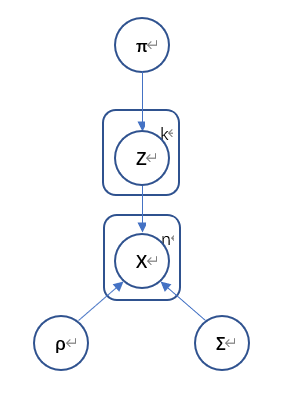
\includegraphics[scale=0.5]{plate.png}
	\end{figure}
	\item 
	令$\gamma_{ji}$表示样本$x_j$由第$i$个高斯混合成分生成的后验概率,即
	\[\gamma_{ji}=p(z_j=i|x_j)=\frac{\pi_i p(x_j|\mu_i,\Sigma)}{\sum_{k=1}^K \pi_i p(x_j|\mu_i,\Sigma)}\]
	我们需要最大化对数似然
	\[LL(D)=\ln\left(\prod_{j=1}^m p(x_j)\right)=\ln\left(\prod_{j=1}^m(\sum_{i=1}^K \mu_i p(x_j|\mu_i,\Sigma)\right)\]
	对$\mu_i$求导,令其为0,得到
	\[\mu_i=\frac{\sum_{j=1}^m \gamma_{ji}x_j}{\sum_{j=1}^m \gamma_{ji}}\]
	对$\Sigma$求导,令其为0,得到
	\[\Sigma=\frac{\sum_{i=1}^K\sum_{j=1}^m \gamma_{ji}(x_j-\mu_i)(x_j-\mu_i)^T}{\sum_{i=1}^K\sum_{j=1}^m \gamma_{ji}}\]
	对$\pi_i$,存在约束条件$\sum_{i=1}^K\pi_i=1$,引入拉格朗日乘子
	\[LL(D)+\mu\left(\sum_{i=1}^K\pi_i=1 \right)\]
	对$\pi_i$求导,令其为0,得到
	\[\pi_i=\frac{1}{m}\sum_{j=1}^m\gamma_{ji}\]
	\item 
	\begin{align*}
		p(x_a|x_b)&=\frac{p(x_a,x_b)}{p(x_b)}\\
				&=\frac{\sum_{k=1}^K\pi_k p(x|k)}{\sum_{k=1}^K\pi_k p(x_b|k)}\\
				&=\sum_{k=1}^K\frac{\pi_k}{\sum_{k=1}^K\pi_k p(x_b|k)}p(x|k)
	\end{align*}
\end{enumerate}
\end{solution}

\section{\textbf{[30pts]}Latent Dirichlet Allocation}
我们提供了一个包含$8888$条新闻的数据集\texttt{news.txt.zip},该数据集中每一行是一条新闻。在该数据集上完成LDA模型的使用及实现。

数据预处理提示:你可能需要完成分词及去掉一些停用词等预处理工作。

在本题中需要完成:
\begin{enumerate}
    \item \textbf{[10pts]}使用开源的LDA库(如scikit-learn),计算给出$K=\{5, 10, 20\}$个话题时,每个话题下概率最大的10个词及其概率。
    \item \textbf{[20pts]}不借助开源库,手动实现LDA模型,计算给出$K=\{5, 10, 20\}$个话题时,每个话题下概率最大的10个词及其概率。
\end{enumerate}
注:需要在报告中描述模型计算的结果,以及如何复现自己的结果,提交的作业中至少应该包含\texttt{lda\_use.py}和\texttt{lda.py}两个文件,分别为使用和不使用第三方库的源码。
\begin{solution}
此处用于写解答(中英文均可)
\begin{enumerate}
	\item 
	下面是使用scikit-learn,K=5的结果,通过命令python lda\_use.py 运行。\\
	K = 5 \\
	Topic 0 \\
	('said', 0.014547103678296461) ('game', 0.010664783557222389) ('team', 0.007327282789613679) ('season', 0.006501587533873795) ('games', 0.005241283867995008) ('players', 0.004893556159632309) ('year', 0.004742545555554349) ('time', 0.004500149785544217) ('second', 0.004373754763936414) ('just', 0.004136235574822283) \\
	Topic 1 \\
	('mr', 0.025243354988931082) ('said', 0.02396280831845908) ('police', 0.006363597881027269) ('court', 0.005758693453298895) ('people', 0.0045078921625961695) ('state', 0.004385900506951129) ('case', 0.004172061354773201) ('law', 0.003613593706641175) ('government', 0.0036079003523033916) ('ms', 0.0034562299248158982) \\
	Topic 2 \\
	('mr', 0.03276749587587859) ('trump', 0.01733843937461631) ('said', 0.014882052215042463) ('clinton', 0.008379556093328685) ('campaign', 0.006765454537565093) ('party', 0.006495318116271615) ('republican', 0.005876439032123827) ('president', 0.0057049311412754305) ('mrs', 0.005320221160296789) ('obama', 0.005208087467918036) \\
	Topic 3 \\
	('said', 0.012107335562967203) ('mr', 0.00838126834273995) ('new', 0.006707796816816145) ('like', 0.006658289994544992) ('ms', 0.005387566746217388) ('people', 0.0038744003571985) ('just', 0.003710731544301894) ('time', 0.003419096976985942) ('years', 0.0029820956325783948) ('york', 0.0029693952919174027) \\
	Topic 4 \\
	('said', 0.015298604016865511) ('percent', 0.006557997882199597) ('company', 0.005516070398827582) ('year', 0.005414792495510575) ('new', 0.005286566630569417) ('million', 0.004333269658216909) ('people', 0.003696363353549135) ('mr', 0.0036154020960351926) ('united', 0.003499234134963485) ('years', 0.003373632618223284)
	\item 
	下面是使用自己的代码K=5的结果,通过命令python lda.py 运行。因为使用吉布斯采样,需要运行非常久。\\
	K = 5 \\
	Topic 0 \\
	('said', 0.020471124261831834) ('mr', 0.004997150625822401) ('year', 0.003898997658105603) ('united', 0.003401223775011751) ('game', 0.0033818119801278684) ('american', 0.0032681143243794117) ('time', 0.003215425166837444) ('season', 0.003205719269395503) ('home', 0.002673281466866146) ('new', 0.00263168476354354) \\
	Topic 1 \\
	('mr', 0.017705976736362535) ('said', 0.01586259421698138) ('percent', 0.007083391173524325) ('company', 0.005421345469143353) ('year', 0.004791043712177205) ('new', 0.004173247942452449) ('court', 0.003930631789969448) ('law', 0.0039068704142108035) ('state', 0.003864350057590071) ('government', 0.003799318923934834) \\
	Topic 2 \\
	('mr', 0.025400077093756086) ('said', 0.014705021037333264) ('trump', 0.011218094966976358) ('clinton', 0.005283510244888452) ('party', 0.004597021674786936) ('people', 0.00456841798436604) ('campaign', 0.004007240819917975) ('new', 0.00378113545754327) ('president', 0.0036231341199802224) ('republican', 0.003575461302612062) \\
	Topic 3 \\
	('said', 0.01344626672711545) ('like', 0.005465951146800407) ('just', 0.004629174968284569) ('time', 0.0044448689611195046) ('city', 0.0036726671500775564) ('mr', 0.0035071953334257105) ('new', 0.003425132074760974) ('year', 0.003251588462174892) ('people', 0.0029865644956674634) ('world', 0.0029771474004108545) \\
	Topic 4 \\
	('said', 0.01086943954492492) ('new', 0.008503110784524056) ('like', 0.007286545455479747) ('mr', 0.007186342608948114) ('ms', 0.006956389922676803) ('people', 0.004090331581496388) ('years', 0.003324679061844426) ('york', 0.003241176689734732) ('work', 0.002918729068203453) ('time', 0.0027144694195043555) \\
\end{enumerate}
\end{solution}
\newpage
\bibliography{ref}
\bibliographystyle{abbrvnat}
\end{document}